\chapter{Ontwerp}

Nu alle deel vragen beantwoord zijn in de Analyse kan er verder gegaan worden met het ontwerpen van de werking van het XILINX bord.

\section{Textueel ontwerp van het programma}

De volgende elementen moeten ontworpen en gerealiseerd worden:
\begin{enumerate}
	\item De clock naar beneden schalen zodat de Leds door mensen te zien zijn
	\item De S88 Signalen moeten nagebootst worden
\end{enumerate}

In dit hoofdstuk zal het ontwerpen plaatsvinden, dus in woorden uitgelegd wat er gedaan moet worden, en in het hoofdstuk realiseren wordt het in VHDL gerealiseerd.

\clearpage
\section{Custom Clockrate genereren}

Het eerste wat gedaan moet worden is de clockrate naar beneden schalen, dit wordt gedaan omdat de normale clockrate $\SI{50}{\mega\hertz} $ is.
\\\\
Als een Led met deze frequentie zou knipperen is dat te hoog om met een menselijk oog waar te kunnen nemen, hierom zal de clockrate intern verlaagt moeten worden.
\\\\
Dit zal gebeuren door middel van een interne timer, die iedere clocktick met één verhoogd wordt.
\\\\
Op het moment dat deze timer, die vanaf dit moment TimingCounter genoemt zal worden, een waarde van ${5} \times {10}^5$ bereikt zal er een andere variabele genaamt TijdseenheidCounter met \'e\'en verhoogd worden. 
\\\\
Er zal een Case statement gebruikt worden met als variable de TijdseenheidCounter, en hiermee zal er op elk tijdseenheid de juiste actie uitgevoerd worden.
\clearpage
	\section{De S88 Signalen}

In de Analyze in de sectie "Hoe werkt een s88 protocol" is reeds uitgelegd hoe het s88 protocolr werkt. 
\\
Hier is uit af te leiden dat er door er gebruikt gemaakt wordt van de volgende I/O poorten:

\begin{itemize}
	\item CLOCK
	\item DATA-OUT
	\item LOAD
	\item RESET
\end{itemize}

Het ontwerpen van deze signalen wordt opgesplitst in twee secties, De initialisatie en het daadwerkelijke uitlezen van het schuifregister.

\section{Initialisatie van het schuifregister}


De volgorde van deze signalen wordt beschreven in onderstaande image.
\begin{figure}
	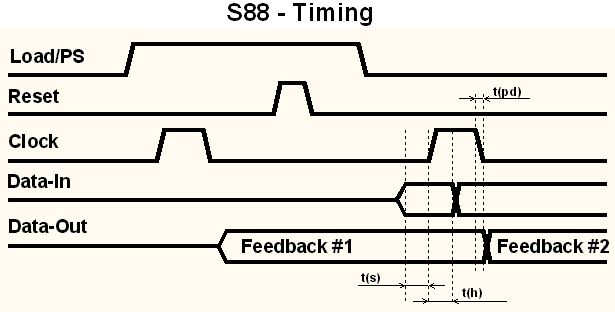
\includegraphics[scale=0.9]{./img/s88timing.png}
	\caption{S88 timing}
\end{figure}


Deze image geeft aan welke poorten wanneer op een logisch 1 gezet moeten worden. Als voorbeeld, de lijn onder Load/PS is de lijn die bij Load hoort. In het begin geeft de lijn een logisch 0 weer, de stijding betekent dat daar de poort op een logisch 1 gezet wordt.
\\\\
Van de poorten Load/PS, Reset en Clock is een UML activiteiten diagram gemaakt, dit is gedaan zodat de volgorde van de signalen overzichtelijker weer te geven is.
\\\\
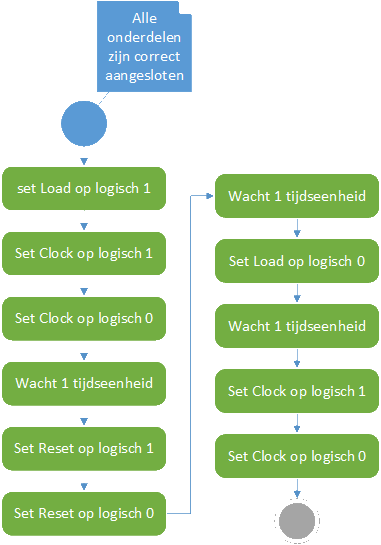
\includegraphics[scale=0.8]{./img/activity.png}
\\\\
Hierin staat één tijdseenheid voor één seconde en is de duur van elke opdracht gelijk aan één tijdseenheid, dus één seconde.\\
Het moet gelezen worden door middel van de pijlen waarin er bovenaan begonnen met lezen wordt bij de blauwe cirkel.\\
Er mag alleen begonnen aan de opdracht als "Alle onderdelen zijn correct aangesloten" waar is, anders heeft het uitvoeren van de in de diagram beschreven opdrachten geen zin.
\\\\
Als er dus gecontroleerd is dat alles correct aangesloten is kan er begonnen worden met de eerste opdracht, in dit geval "Set Load op logisch 1". Nadat deze opdracht uitgevoerd is kan er verdergegaan worden met de opdracht die door middel van de pijl verbonden is, in dit geval "Set Clock op logisch 1". Zo wordt er verdergegaan totdat alle opdracht uitgevoerd zijn, als alle opdrachten uitgevoerd zijn is het schuifregister succesvol geïnitialiseerd.
\newpage
\section{Uitlezen van het Schuifregister}

Nadat de initialisatie voltooid is kan er begonnen worden met het uitlezen van het schuifregister. 
Zoals is beschreven in de analyse kan het schuifregister op de volgende manier uitgelezen worden, er wordt één tijdseenheid een logische 1 op Clock gezet, op de falling-edge van de Clock komt de volgende bit van het schuifregsiter op Data-Out gezet.
\\\\
Dus nadat de Data-Out uitgelezen te hebben kan door middel van de Clock één tijdseenheid een logisch 1 te maken het volgende bit uit het schuifregister op de Data-Out gezet worden. En op die manier kan het hele schuifregister uitgelezen worden.


\begin{flushleft}
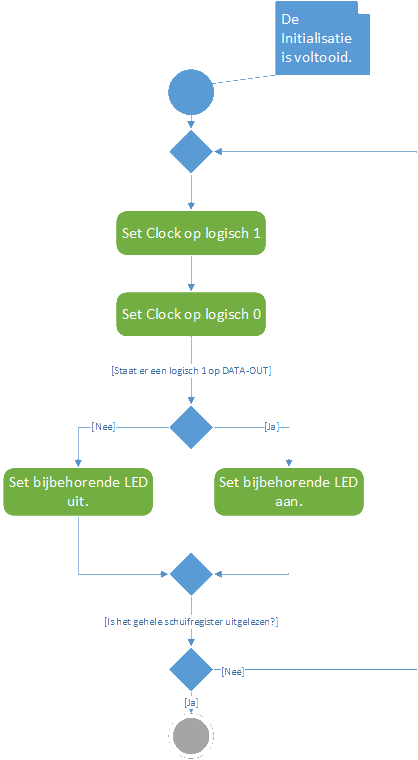
\includegraphics[scale=0.8]{./img/activity2.png}
\end{flushleft}


Wat hier niet goed weergegeven is is dat het net zo vaak uitgevoert zal worden totdat alle bits uit het schuifregister uitgelezen zijn, normaal gesproken wordt dit gedaan met een Loop maar omdat er bij de vereisten al vastgelegd is dat er gebruik gemaakt zal worden van de hardware beschrijving taal VHDL zal dit anders verlopen.\\\\
VHDL beschikt namelijk wel degelijk over een loop maar deze zal hier niet gebruikt worden, de redenatie hierachter is als volgt. Alle elementen worden geclockt op de CustomClock. Een loop kan niet geclockt worden en zal dus zal niet goed kunnen omgaan met de rest van het systeem.
\\\\
Wat er wel gedaan zal worden is het volgende, vanaf het moment dat de initialisatie voltooid is zal er om de tijdseenheid de Clock voor één tijdseenheid logisch 1 gemaakt worden. De tijdseenheid die er dan tussen zit zal gebruikt worden om Data-Out uit te lezen.
Dit zal net zo lang doorgaan totdat alle bits uit het schuifregister door het systeem uitgelezen zijn.